% 1977 年广西卷第 5 题：抛物线拱桥 x²=−9y，顶点在原点、开口向下，
% 跨度 AB=12 米（A(−6,−4)、B(6,−4)），撑梁 C1D1…C4D4 竖直，桥面线 y=−4（按源卷第 4 页布局）
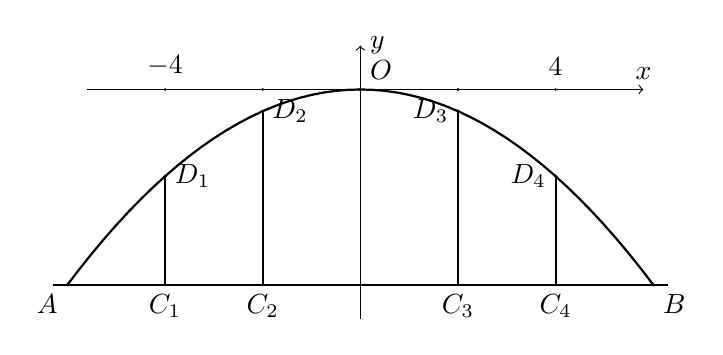
\begin{tikzpicture}[scale=0.62]
  % 坐标轴
  \draw[->] (-5.6,0) -- (5.8,0) node[above] {$x$};
  \draw[->] (0,-4.7) -- (0,0.9) node[right] {$y$};
  \fill (0,0) circle (1.1pt) node[above right] {$O$};
  % 抛物线 y = -x^2/9（顶点在原点，开口向下）
  \draw[thick, domain=-6:6, samples=49] plot (\x, {-\x*\x/9});
  % 桥面线（弦 AB 所在水平线）
  \draw[thick] (-6.3,-4) -- (6.3,-4);
  \fill (-6,-4) circle (1.1pt) node[below left] {$A$};
  \fill (6,-4) circle (1.1pt) node[below right] {$B$};
  % 四根撑梁（x=±2、±4）
  \foreach \i/\xx in {1/-4, 2/-2, 3/2, 4/4} {
    \pgfmathsetmacro{\yy}{-\xx*\xx/9}
    \draw[thick] (\xx,-4) -- (\xx,\yy);
    \fill (\xx,-4) circle (1pt) node[below] {$C_{\i}$};
    \pgfmathtruncatemacro{\side}{\xx>0 ? -1 : 1}
    \ifnum\side<0
      \fill (\xx,\yy) circle (1pt) node[left] {$D_{\i}$};
    \else
      \fill (\xx,\yy) circle (1pt) node[right] {$D_{\i}$};
    \fi
  }
  % x 轴刻度点与标注（−4 与 4）
  \foreach \xx in {-4,-2,2,4} { \fill (\xx,0) circle (0.9pt); }
  \node[above] at (-4,0.08) {$-4$};
  \node[above] at (4,0.08) {$4$};
\end{tikzpicture}
